\chapter{Feature Engineering}

Cette partie décrit la transformation des données brutes en jeux de données exploitables par les modèles de Machine Learning. L'objectif n'est pas seulement d'ajouter un grand nombre de variables, mais de construire des variables cohérentes avec la physique du phénomène étudié et compatibles avec une prédiction en temps réel. Chaque variable explicative doit donc être disponible à l'instant de prédiction ou dans le passé. Cette règle est essentielle pour éviter toute fuite d'information depuis le futur.

La cible du projet est la variabilité future de la production photovoltaïque normalisée, mesurée à l'horizon de 30 minutes. En pratique, le modèle cherche à prédire l'amplitude de la variation future plutôt que son signe. La formulation retenue est :

\begin{equation}
target(t) = |TCH\_solaire(t + \Delta t) - TCH\_solaire(t)|
\end{equation}

Avec : $\Delta t = 30 minutes$

Cette définition permet de se concentrer sur les épisodes de stabilité ou d'instabilité de la production solaire. Une valeur élevée de la cible correspond à une variation importante de la production sur le prochain pas de temps, ce qui est particulièrement utile pour anticiper les rampes photovoltaïques.

\begin{figure}[htbp]
    \centering
    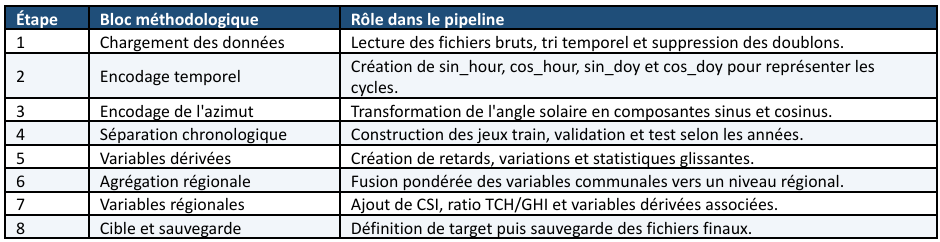
\includegraphics[width=0.9\textwidth]{img/pipe_fe.png}
    \caption{Chaîne générale du feature engineering.}
    \label{fig:pipe_fe}
\end{figure}

\section{Objectif et principe général}

Le feature engineering part du jeu de données principal couvrant plusieurs années d'observations. Les variables disponibles incluent notamment des informations de production, des variables radiatives, des variables météorologiques, des variables solaires géométriques et des observations associées à plusieurs points représentatifs de la région PACA. Le notebook identifie cinq points d'intérêt, repérés par les préfixes \textit{cru}, \textit{sel}, \textit{svt}, \textit{bra} et \textit{eyg}. Cette organisation permet d'automatiser les mêmes transformations sur chaque point.

Un principe directeur est conservé tout au long de la préparation : les transformations doivent reproduire les conditions d'une utilisation future du modèle. Ainsi, les variables retardées et les statistiques glissantes sont construites à partir du passé. Les variables qui utiliseraient directement la valeur future de la production ne sont pas intégrées comme variables explicatives.

\section{Encodages temporels et angulaires}

Les phénomènes photovoltaïques sont fortement cycliques. La production dépend de l'heure de la journée, de la position dans l'année et de la position apparente du soleil. Utiliser directement l'heure ou le jour de l'année comme des entiers créerait des discontinuités artificielles : par exemple, 23 h et 0 h sont proches dans la réalité, mais éloignés numériquement. Pour éviter ce problème, les variables cycliques sont encodées sous forme de sinus et de cosinus.

\begin{figure}[htbp]
    \centering
    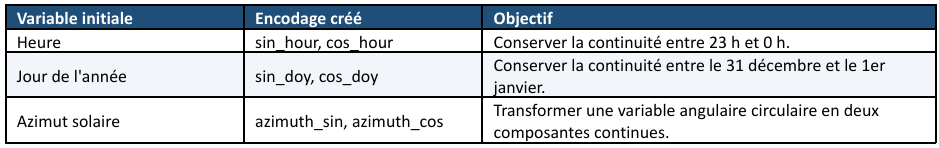
\includegraphics[width=0.9\textwidth]{img/tab2.png}
    \caption{Encodages cycliques utilisés pour les variables temporelles et angulaires.}
    \label{fig:tab2}
\end{figure}

\begin{figure}[htbp]
    \centering
    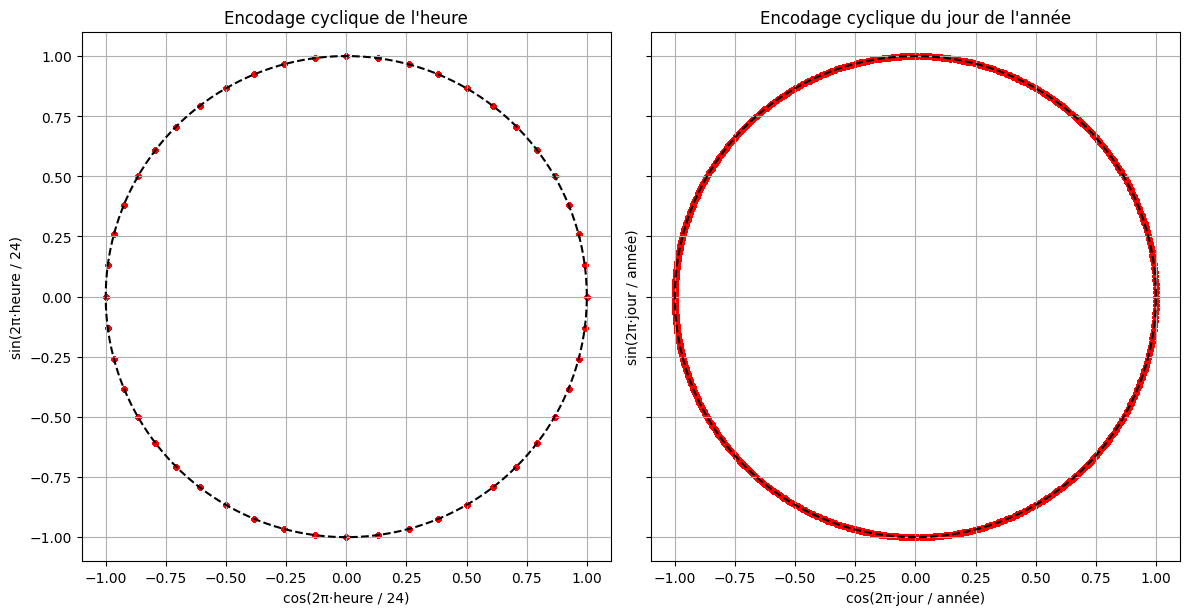
\includegraphics[width=0.9\textwidth]{img/cycle1.png}
    \caption{Vérification de l'encodage cyclique de l'heure et du jour de l'année.}
    \label{fig:cycle1}
\end{figure}

\begin{figure}[htbp]
    \centering
    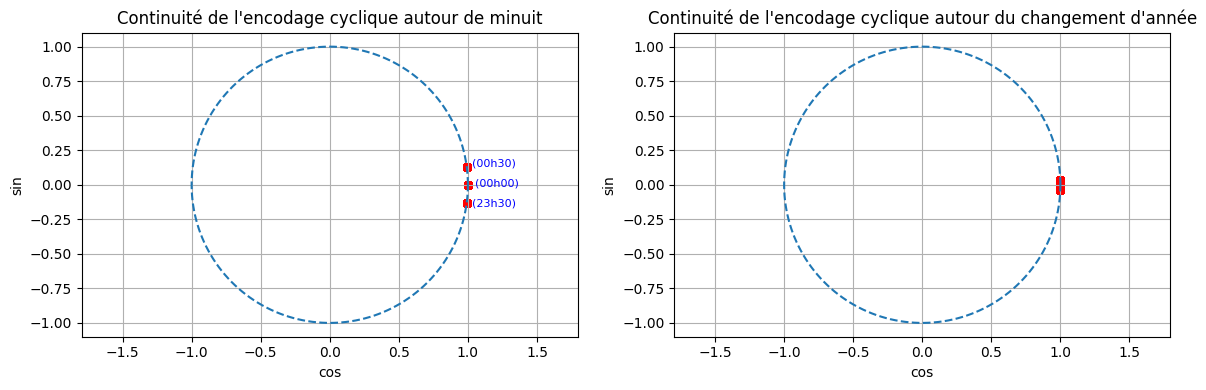
\includegraphics[width=0.9\textwidth]{img/cycle2.png}
    \caption{Continuité autour de minuit et du changement d'année.}
    \label{fig:cycle2}
\end{figure}


Les figures montrent que les points se placent sur un cercle unité. Cette représentation garantit que deux instants proches dans le cycle restent proches dans l'espace des variables, même lorsqu'ils se situent de part et d'autre d'une frontière numérique. Cet encodage est particulièrement important pour les modèles d'arbres et les modèles linéaires, car il évite d'introduire une rupture artificielle dans les données.

\section{Variables dérivées communales}

Après les encodages cycliques, le notebook ajoute des variables décrivant la dynamique récente des grandeurs physiques. La variabilité solaire à court terme est souvent liée à des changements rapides d'irradiance, à la nébulosité et à la variation récente de la production. Pour cette raison, plusieurs familles de variables sont enrichies par des retards, des variations instantanées et des statistiques glissantes.

\begin{figure}[htbp]
    \centering
    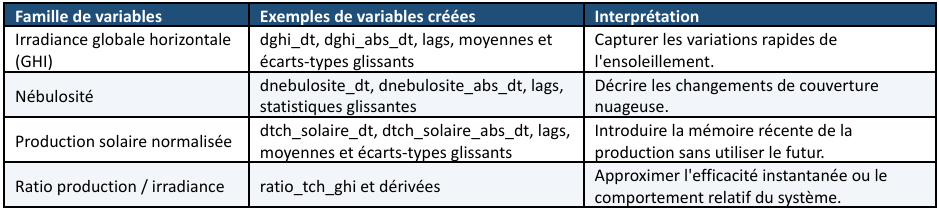
\includegraphics[width=0.9\textwidth]{img/tab3.png}
    \caption{Exemples de variables dérivées construites dans le notebook.}
    \label{fig:tab3}
\end{figure}

Les variables de retard permettent au modèle d'observer la mémoire courte du système. Les variations absolues mesurent l'intensité des changements récents, tandis que les statistiques glissantes sur deux heures résument l'état récent du ciel et de la production. Cette combinaison est pertinente pour un problème de variabilité : il ne suffit pas de connaître la valeur actuelle d'une variable, il faut aussi connaître la dynamique qui précède cette valeur.

Le notebook applique les mêmes transformations aux ensembles d'entraînement, de validation et de test. Ce choix assure que les trois jeux de données possèdent la même structure de colonnes. Il facilite également la reproductibilité du pipeline et limite le risque d'erreurs manuelles.

\section{Nettoyage, séparation temporelle et sauvegarde intermédiaire}

Les retards et les fenêtres glissantes introduisent naturellement des valeurs manquantes au début des séries temporelles. Ces lignes sont supprimées après la création des variables. Les colonnes sont ensuite triées afin de rendre les fichiers plus lisibles et de faciliter les vérifications.

\begin{figure}[htbp]
    \centering
    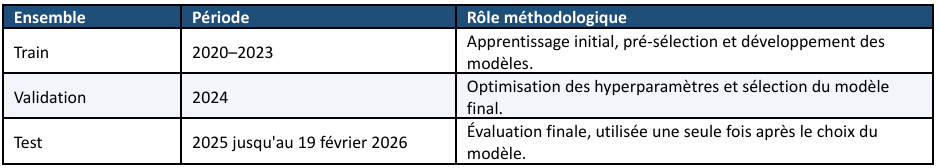
\includegraphics[width=0.9\textwidth]{img/tab4.png}
    \caption{Séparation chronologique des données pour éviter la fuite temporelle.}
    \label{fig:tab4}
\end{figure}


Le choix d'une séparation temporelle est fondamental. Un découpage aléatoire mélangerait des observations passées et futures, ce qui pourrait conduire à une évaluation trop optimiste. La validation sur 2024 et le test sur une période postérieure reproduisent une situation plus réaliste : entraîner le modèle sur le passé et vérifier sa capacité à généraliser dans le futur.

\clearpage

\section{Agrégation régionale et variables complémentaires}

Le notebook construit d'abord une version détaillée avec les variables de cinq points représentatifs. Cette représentation est riche, mais elle augmente fortement le nombre de colonnes. Pour la modélisation finale, une version régionale est ensuite créée. Les variables communales présentes pour les cinq points sont agrégées au niveau régional, puis les colonnes communales devenues inutiles sont supprimées.

Cette étape réduit la dimension du problème tout en conservant une information spatiale synthétique. Elle est cohérente avec l'objectif du projet, qui consiste à prédire la variabilité régionale de la production solaire plutôt que la dynamique d'une seule commune.

\begin{figure}[htbp]
    \centering
    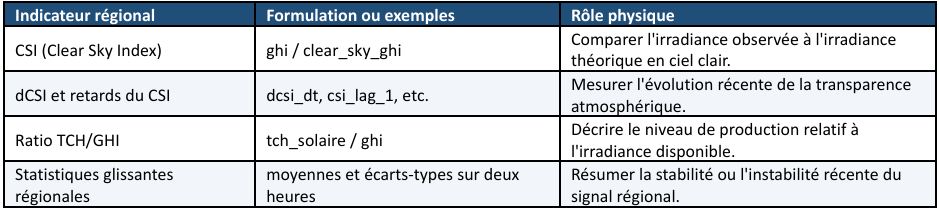
\includegraphics[width=0.9\textwidth]{img/tab5.png}
    \caption{Variables régionales complémentaires ajoutées après l'agrégation.}
    \label{fig:tab5}
\end{figure}

Le CSI est particulièrement utile : il donne une indication de l'écart entre les conditions réelles et les conditions de ciel clair. Des variations importantes de CSI peuvent correspondre à des passages nuageux ou à des transitions atmosphériques rapides, souvent associées à des variations de production. Le ratio TCH/GHI complète cette information en reliant directement la production solaire à l'irradiance disponible.

\section{Bilan du feature engineering}

Chaque ligne contient les informations disponibles au temps présent ou dans le passé, et la cible indique l'amplitude de la variation qui se produira au pas suivant.

À l'issue de cette étape, les fichiers régionaux finaux sont prêts pour le notebook de modélisation. Cette transition marque le passage d'une logique de préparation des données vers une logique d'évaluation et de sélection de modèles.
